\lez{16}{23-04-2020}{}
Facciamo un esempio per vedere come nelle stelle le reazioni nucleari avvengono lentamente, prendiamo il centro del sole ($T_{c,\odot}=15\cdot 10^6$ K), il fattore astrofisico $S(E)$ della reazione $p+p$ nel sole è:
\[
S_{c,p+p}=S_0=3,89\cdot 10^{-25} \text{MeV}\text{ barn}
.\] 
Quindi si ottiene per la $p+p$:
\[
\left<\sigma v\right>\approx 10^{-43} \text{cm}^3 /\text{s}
.\] 
Nota questa quantità possiamo calcolare il numero di protoni per unità di volume nel centro del sole $n_p \sim 10^{26}$ cm$^3$ in modo tale da ottenere il reaction rate:
\[
n_{pp} = \frac{n_p^2
}{2}\sim 10^9 \text{cm}^3\text{ s}
.\] 
Per capire la lentezza di tale reazione possiamo confrontarla con il rate di collisioni $\sigma_\text{coll} v$,possiamo farlo prendendo la sezione d'urto geometrica, la velocità quella termica dei protoni:
\[
v = \sqrt{\frac{3kT}{m_p}}\approx 6\cdot 10^7 \text{cm}/\text{s}
.\] 
Facendo il rapporto tra questo Rate di collisioni e quello di reazione nucleare della $p+p$ scopriamo che:
\[
\frac{\left<\sigma v\right>}{\sigma_\text{coll} v} \sim 10^{-25}
.\] 
Che è molto basso, quindi la stragrande maggioranza dei protoni che si urtano nel centro del sole non fa reazione nucleare perché non supera la barriera coulumbiana (fa solo scattering). \\
È ancora più piccola invece la frazione di protoni che, superata la barriera coulumbiana tramite effetto tunnel riuscirà a fare le reazioni nucleari. \\
Le reazioni nucleari all'interno delle stelle sono quindi molto poco efficienti.\\
Un altro modo per vedere questa lentezza è provare a quantificare il tempo scala in cui viene modificata la composizione chimica. Se studiamo sempre la $p+p$ abbiamo una reazione che consuma idrogeno, possiamo vedere come cambia il numero di protoni per unità di tempo (supponendo che i protoni vengano consumati solo dalla $p+p$)
\[
    \frac{\text{d} n_p}{\text{d} t} = -n_{pp}\left(1+\delta_{ij}\right) =
    -\frac{n_p}{\tau_p}
.\] 
Dove $\tau_p$  è la vita media dei protoni, confrontando $n_{pp}$  con quello visto sopra scopriamo che:
\[
\tau_p = \frac{1}{n_p\left<\sigma v\right>} \sim 10^{17} \text{ s}
.\] 
Dove abbiamo inserito i dati del centro del sole $n_p \sim 10^{26}$, $\left<\sigma v\right>\sim 10^{-43}$. \\
Il tempo ottenuto è dell'ordine di 3 miliardi di anni, quindi deve passare parecchio tempo prima che si bruci un protone\ldots\\
Abbiamo considerato fin'ora delle reazioni come se non ci fossero elettroni in circolazione (come se i nuclei fossero nudi). Ovviamente nelle regioni centrali delle stelle i nuclei sono ionizzati, tuttavia gli elettroni liberi sono ancora presenti. I nuclei sono immersi in un background di elettroni, tali elettroni schermeranno i nuclei rendendo più bassa la barriera coulumbiana.\\
Possiamo vedere che il potenziale di un nucleo si trasforma come:
\[
\frac{Ze}{r} \to \frac{Ze}{r} e^{-r /\lambda_D}
.\] 
Dove $\lambda_D$  è la lunghezza d'onda di Debye:
\[
    \lambda_D = \sqrt{\frac{kT}{4\pi e^2 \sum_{}^{} n_e^i\left(Z_i+1\right)}} 
.\] 
Dove 
\[
n_e^i = \frac{\rho}{m_H}\frac{X_iZ_i}{A_i}
.\] 
Nelle stelle solitamente siamo in una situazione di schermo debole: 
\[
\lambda_D\gg r_\text{min} 
.\] 
Dove $r_\text{min}$ è la distanza minima raggiunta dalle particelle nell'urto
\[
\frac{\lambda_D}{r_\text{min}} \sim  50-100
.\] 
quindi si ha sempre che $r /\lambda_D \sim 0$. Gli elettroni allora non saranno distribuiti in modo omogeneo ma saranno distribuiti attorno ai nuclei e tenderanno a schermare in parte il campo di questi ultimo, tuttavia lo schermaggio è molto debole ad abbiamo solo una piccola variazione dal campo coulumbiano. \\
Le formule viste sopra restano giuste, vanno solo corrette per un fattore:
\[
f = e^{E_D /kT}
.\] 
In cui abbiamo introdotto l'energia di Debye
\[
E_D = \frac{Z_iZ_j e^2}{\lambda_d}
.\] 
Grazie al fattore $f$ il reaction rate viene leggermente amplificato.\\
Abbiamo visto che in caso di schermo non degenere in assenza di sorgenti nucleari (o con sorgenti non in grado di compensare la luminosità) allora sappiamo che:
\[
    L>0 \implies \dot{\Omega}<0 \ \dot{T} > 0
.\] 
Ora sappiamo anche che, poichè la barriera coulmbiana è grande rispetto a $kT$ abbiamo reazioni in cui il $\left<\sigma v\right>$  dipende in modo sensibile dalla temperatura:
\[
\left<\sigma v\right>\sim T^n
.\] 
Queste due condizioni insieme formano il famoso termostato stellare.
\subsection{Riassunto sui processi di evoluzione stellare}%
\label{sub:Riassunto sui processi di evoluzione stellare}
La stella alla nascita sarà troppo fredda per le reazioni nucleari, per questo contrae ed aumenta la temperatura; se si raggiunge la temperatura sufficiente per l'innesco $p+p$ allora si passa ad una situazione di lungo equilibrio in cui si ha termostato stellare (stop-nucleare).\\
Successivamente le fusioni termonucleari modificano la composizione chimica aumentando il peso molecolare aumenta. Aumentano tale peso la stella continua a contrarsi con tempi scala nucleari.\\
Una volta che finisce l'idrogeno se la stella non ha la temperatura sufficiente ad innescare subito la reazione successiva (He) torna sotto la guida del Viriale ricominciando a contrarsi e scaldarsi. \\
La durata dello stop nucleare dipende dal quantitativo di combustibile e dall'energia rilasciata per unità di energia rilasciata per unità di massa da tale combustibile.\\
Visto che nella combustione (H$\to $ He) viene rilasciato lo 0.7\% dell'energia a riposo (80\% di tutta l'energia che può essere rilasciata da tutte le reazioni nucleari) questa fase sarà molto più lunga della successiva (che rilascia lo 0.0065 \% dell'energia a riposo). \\
Anche nella eventualità in cui la luminosità sia la stessa dobbiamo aspettarci che la seconda fase sia più breve della prima. \\
Nelle reazioni successive la situazione sarà ancora più vistosa (avviciniandoci al picco del ferro l'energia rilasciata diminuisce sempre di più), dobbiamo allora aspettarci che la durata delle fasi sia molto diversa e che andando verso il picco tali durate diminuiscano.\\
Vedremo che questa cosa sarà accentuata ancora di più dal fatto che la luminosità della stella aumenta fase dopo fase, quindi serve sempre più energia.\\
Il termostato può essere interrotto se la stella diventa degenere (in tutta la stella nelle nane bianche o in una regione nelle giganti rosse), in questo caso la pressione è dominata dagli elettroni degeneri. Nel caso di degenerazione completa la pressione dipenderà unicamente dalla densità e non dalla temperatura. \\
Se accendiamo una reazione nucleare in un ambiente elettronicamente degenere entriamo in una situazione pericolosa: la stella non reagisce più con una espansione alle reazioni, diminuendo la temperatura e portando il tutto all'equilibrio perché la pressione è indipendente dalla temperatura. Tutta l'energia liberata dalle reazioni viene convertita in energia cinetica dei nuclei di conseguenza la temperatura aumenta ulteriormente. \\
Si innesca così un meccanismo auto-alimentante che porta a liberare una enorme quantità di energia ed aumentare esponenzialmente la temperatura in pochissimo tempo, qui siamo vicini ad una bomba: questo fenomeno è detto Flash e porta a far esplodere la stella.
\subsection{Catena p-p.}%
\label{sub:Catena p-p.}
Abbiamo visto che il fattore di penetrazione di Gamov decresce esponenzialmente con la carica, quindi ci dobbiamo aspettare che la probabilità di superare la barriera coulumbiana più alta possibile si dovrebbe avere tra due protoni. 
Tuttavia adesso vedremo che la $p+p$ non è la prima reazione che avviene nelle stelle, la prima reazione che avviene è la $p+D$ (Deuterio).\\
Dal punto di vista della barriera coulumbiana l'altezza è la stessa, tuttavia la massa ridotta della $p+D$ sarà maggiore della $p+p$. 
Quindi vista la forma del fattore di penetrazione di Gamow:
\[
    e^{-2\pi\eta}
.\] 
Dove: 
\[
\eta  = \frac{Z_iZ_j e^2}{\hbar  v} 
= \sqrt{\frac{m}{2}}\frac{Z_iZ_je^2}{\hbar \sqrt{E}}
.\] 
Il fattore di penetrazione di Gamov sarà più basso per la $p+D$ rispetto alla $p+p$. Questo ci dice anche il superamento della barriera coulumbiana avviene con maggiore probabilità per la $p+p$  che per la $p+D$.\\
Tuttavia la $p+D$  avviene a temperature più basse della $p+p$ per via della sezione d'urto: questa non dipende soltanto dalla penetrazione della barriera coulumbiana ma dipende anche dalle proprietà nucleari
\[
    \sigma (E) = \frac{S(E) }{E}e^{-2\pi\eta}
.\] 
È il fattore astrofisico che in questo caso ribalta la situazione. Il motivo è che la $p+p$ è una reazione debole!
\[
p+p\to D +e^+ +\nu
.\] 
Un protone deve essersi convertito in un neutrone: deve essere avvenuta una reazione debole. 
Come abbiamo sempre detto per le interazioni deboli la sezione d'urto è minore rispetto alle reazioni forti o EM. Nel caso della $p+D$ si ha una cattura radiativa:
\[
    p+D \to {}^3He + \gamma
.\]  
Quindi il fattore astrofisico in questo caso è molto più grande rispetto alla interazione debole.\\
Questo fa si che nel processo di contrazione di stella neonata la prima reazione che si può attivare è la $p+D$ a temperature dell'ordine $T\sim 10^6$ K, a tale temperatura la $p+p$ è del tutto trascurabile.\\
Vedremo che questa fase di combustione non riesce a durare tanto poiché nella materia della stella non vi è molto deuterio disponibile.\\
La stella continua la sua contrazione bruciando gli altri elementi leggeri (${}^7$Li, Be, B, \ldots) che sono poco abbondanti. \\
A temperature dell'ordine di $T\sim 6\cdot 10^6$ K allora si innesca la $p+p$. \\
Quando si attiva tale reazione si ricomincia a produrre Deuterio, quindi diventa possibile ripetere la $p+D$ (la temperatura c'è, quindi si può). Visti i prodotti di reazione di quest'ultima avremo che si produce ${}^3$He e si accumula, quando la temperatura evolve poi si raggiungeranno le temperature necessarie a fondere l'He:
\[
    {}^3\text{He}+{}^3\text{He}\to {}^4\text{He}+2p
.\] 
Questa avviene quando la temperatura è $T\approx_8\cdot 10^6$ K.\\
Vediamo che questa catena converte l'idrogeno in He, il nome di tale catena è $p-p \text{ \rom{1}}$. Questa è la sorgente della maggior parte della luminosità del sole.\\
Quando si raggiungono temperature dell'ordine dei $15\cdot 10^6$ K allora diventa attiva la seguente reazione
\[
    {}^3\text{He} + {}^4\text{He}\to {}^7\text{Be}+\gamma
.\] 
A questo punto si ha una biforcazione delle possibili reazioni nella stella a seconda di cosa succede al ${}_7$Be (si dice un Branching Ratio che favorirà uno dei due rami a seconda della temperatura):
\begin{itemize}
    \item $p-p$ \rom{2}.
    \item $p-p$ \rom{3}
\end{itemize}
Il berillio è instabile per cattura $K$: un atomo di ${}^7$Be con un tempo di dimezzamento di 57 giorni ($\tau\sim 57$d) cattura un elettrone dell'orbita $K$ cambiando di natura:
\[
    {}^7\text{Be}+e^-\to {}^7\text{Li}+\nu
.\] 
Nelle stelle tale Berillio sarà completamente ionizzato, quindi l'elettrone arriverà dal Background di elettroni liberi attorno a lui. Questo processo è quello favorito fino alle temperature $T\sim 15 \cdot 10^6$ K. A questo punto il ${}^7$Li cattura un protone formando ${}^8$Be:
\[
    {}^7\text{Li}+p\to {}^8\text{Be}
.\] 
Il ${}^8$Be è instabile, decade in due particelle $\alpha$ in circa $10^{-16}$ s. Questo primo processo è detto $p-p$\rom{2}.\\
Attualmente nel sole questo processo produce circa il 10\% dell'energia totale, il 90\% è prodotto dalla $p-p$ \rom{1}.\\
A temperature di circa $T\sim 20\cdot 10^6$ K il rate del processo 
\[
    {}^7\text{Be}+p\to {}^8\text{B}+\gamma
.\] 
inizia a diventare non trascurabile, quindi oltre queste temperature prende piede anche questa reazione. Il ${}^8$B è instabile e fa $\beta^+$:
\[
    {}^8\text{B}\to {}^8\text{Be}+e^-+\nu
.\] 
A questo punto abbiamo di nuovo che il ${}^8$Be produce le due particelle $\alpha$, questa che abbiamo appena descritto è la $p-p$ \rom{3}.\\
I 3 processi descritti adesso formano la catena $p-p$, in tale catena qualunque sia il processo (la strada seguita) alla fine devo aver fatto:
\[
    4p\to {}^4\text{He}
.\] 
Quindi 2 protoni in un modo o nell'altro devo convertirli in 2 neutroni. In questo processo per ogni nucleo di ${}^4$He devo aver prodotto 2 neutrini. Questi neutrini, avendo una sezione d'urto molto bassa con la materia stellare possono attraversare il sole senza interagire portando via energia alla struttura.\\
La fuga di questi neutrini comporta una variazione del $Q$-valore, sarà necessario togliere da quest'ultimo l'energia dei neutrini prodotti (a noi interessa l'energia ridistribuita alla stella).\\
Nel caso della $p-p$ i neutrini della $p-p$ \rom{1} portano via in media il 2\% dell'energia totale, quelli della $p-p$ \rom{2} il 4\%, quelli della $p-p$ \rom{3} portano via circa il 28\%. \\
Nella catena $p-p$ abbiamo alcuni elementi che vengono prodotti da una reazione e poi distrutti da un'altra (il Deuterio), questi tipi di elementi prendono il nome di Elementi secondari per la catena. Dobbiamo aspettarci che questi elementi secondari raggiungano una situazione di equilibrio.\\
Possiamo allora chiederci come si calcola l'abbondanza all'equilibrio di tali elementi secondari,  nel caso del Deuterio abbiamo un rate di produzione dovuto alla $p+p\to \ldots$ ed un rate di distruzione dovuto alla $p+D\to \ldots$. Per studiare come cambia l'abbondanza di Deuterio è necessario fare la differenza di questi due Rate che sappiamo scrivere:
\[
\frac{\text{d} n_{D}}{\text{d} t} = \frac{n_p^2}{2}\left<\sigma_{p-p}v\right>
- n_pn_D \left<\sigma_{p-D}v\right>
.\] 
Se la reazione avviene per un tempo abbastanza lungo dobbiamo aspettarci che si instauri un equilibrio (situazione stazionaria), in tal caso:
\[
    \left(\frac{n_D}{n_p}\right)_\text{eq} =
    \frac{1}{2}\frac{\left<\sigma_{p-p}v\right>}{\sigma_{p-D}v}
.\] 
Ci aspettiamo in questo caso che l'abbondanza relativa del deuterio sia molto piccola a causa delle due sezioni d'urto che abbiamo discusso sopra.
\subsection{Ciclo CN-N0}%
\label{sub:Ciclo CN-NO}
Questo è un ciclo (non una catena), tale processo si attiva a temperature dell'ordine di $T\sim 15\cdot 10^6$ K ed ha bisogno per attivarsi di alcuni catalizzatori: C,O,N. Essendo un ciclo possiamo partire a spiegarlo da uno qualsiasi di questi 3, partiamo dal ${}^{12}$C (che determina il ciclo CN) :
\[
{}^{12}\text{C}+p \to {}^{13}\text{N}+\gamma
.\] 
L'azoto a questo punto fa un decadimento $\beta^+$:
\[
{}^{13}\text{N}\to {}^{13}\text{C}+e^+ + \nu
.\] 
Il ${}^{13}$C fa la cattura protonica:
\[
{}^{13}\text{C}+ p \to  {}^{14}\text{N} +\gamma
.\]  
Che a sua volta cattura un protone:
\[
{}^{14}\text{N}+p\to {}^{15}\text{O}+\gamma
.\] 
Ma ${}^{15}$O è instabile $\beta^+$:
\[
{}^{15}\text{O}\to {}^{15}\text{N}+e^++\nu
.\] 
Adesso ${}^{15}$N cattura un protone e si forma un nucleo composto in uno stato eccitiato:
\[
    {}^{15}\text{N}+p \to \left({}^{16}\text{O}^*\right)
    \to {}^{12}\text{C}+\alpha
.\] 
Abbiamo prodotto il nucleo di ${}^{4}$He, inoltre il ${}^{12}$C viene risputato fuori (non è consumato): l'abbondanza relativa dei catalizzatori cambia ma la somma delle abbondanze di questi ultimi resta invariata.\\
Nell'1\% dei casi l'ultima reazione può fare:
\[
    {}^{15}\text{N}+p \to \left({}^{16}\text{O}^*\right)
    \to {}^{16}\text{O}+\gamma
.\] 
Quindi può partire il ciclo CO, questo ciclo si attiva a temperature un po più alte $T\sim 20\cdot 10^{6}$ K.
\[
{}^{16}\text{O}+ p\to {}^{17}\text{F}+\gamma
.\] 
Il ${}^{17}$F decade $\beta^+$  :
\[
{}^{17}\text{F}\to {}^{17}\text{O}+e^++\nu
.\] 
A questo punto ${}^{17}$O cattura un protone
\[
    {}^{17}\text{O}+p\to \left({}^{18}\text{F}\right) 
    \to {}^{14}\text{N}+\alpha
.\] 
Quindi l'azoto viene reinserito nel ciclo CN. Quest'ultima reazione può diramarsi in un secondo caso (molto improbabile):
\[
    {}^{17}\text{O}+p\to \left({}^{18}\text{F}\right)^*
    \to {}^{18}\text{F}+\gamma
.\] 
Questo ${}^{18}$F decade $\beta^+$:
\[
{}^{18}\text{F}\to {}^{18}\text{O}+e^-+\nu
.\] 
L'${}^{18}$O fa la cattura protonica:
\[
{}^{18}\text{O}+p\to \left({}^{19}\text{F}*\right)
.\] 
Ed ancora abbiamo una diramazione, nella maggior parte dei casi fa:
\[
\left({}^{19}\text{F}*\right)\to {}^{15}\text{N}+\alpha
.\] 
Producendo di nuovo un catalizzatore che finisce nel ciclo, in un caso meno probabile abbiamo:
\[
\left({}^{19}\text{F}*\right)\to {}^{19}\text{F}+\gamma
.\] 
Ed il ${}^{19}$F catturerà un $p$  producendo:
\[
{}^{19}\text{F}+p\to {}^{16}\text{O}+\alpha
.\] 
in un caso ancor meno probabile il ${}^{19}$F produce:
\[
{}^{19}\text{F}\to {}^{20}\text{Ne}+\alpha
.\] 
Questa uscita è una eccezione (non produce un catalizzatore con una particella $\alpha$), questa è una perdita per il ciclo che sottrae catalizzatori,
tuttavia quest'ultimo processo è altamente improbabile.\\
Nel piano Z-N i nuclei si dispongono lungo la diagonale, gli elementi che stanno sopra la diagonale saranno instabili perché hanno un eccesso di protoni, quelli che stanno sotto saranno instabili perché hanno un eccesso di protoni. \\
Per questo motivo quelli che stanno sotto avranno la necessità di fare decadimento $\beta^-$ per convertire un protone in un protone. Quelli che sono sopra per tornare nella valle di stabilità dovranno fare viceversa decadendo $\beta^+$. Questo spiega tutte le reazioni $\beta$ viste sopra. \\
È molto importante ricordarsi sia il ciclo CN che il ciclo NO.
\begin{figure}[H]
    \centering
    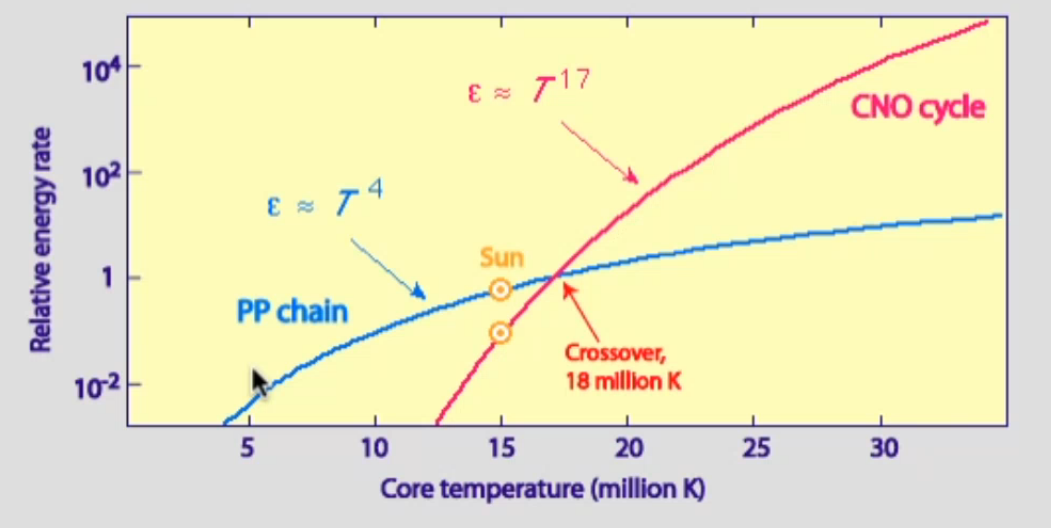
\includegraphics[width=0.7\textwidth]{figures/catene.png}
    \caption{Catene}
    \label{fig:fi}
\end{figure}
\noindent
Notiamo che le pendenze per le due curve sono differenti, infatti nella p-p e nella CN-NO le cariche coinvolte sono differenti.
